\documentclass[14pt]{extbook}
\usepackage{multicol, enumerate, enumitem, hyperref, color, soul, setspace, parskip, fancyhdr} %General Packages
\usepackage{amssymb, amsthm, amsmath, bbm, latexsym, units, mathtools} %Math Packages
\everymath{\displaystyle} %All math in Display Style
% Packages with additional options
\usepackage[headsep=0.5cm,headheight=12pt, left=1 in,right= 1 in,top= 1 in,bottom= 1 in]{geometry}
\usepackage[usenames,dvipsnames]{xcolor}
\usepackage{dashrule}  % Package to use the command below to create lines between items
\newcommand{\litem}[1]{\item#1\hspace*{-1cm}\rule{\textwidth}{0.4pt}}
\pagestyle{fancy}
\lhead{Progress Quiz 8}
\chead{}
\rhead{Version B}
\lfoot{4553-3922}
\cfoot{}
\rfoot{Fall 2020}
\begin{document}

\begin{enumerate}
\litem{
Determine the horizontal and/or oblique asymptotes in the rational function below.\[ f(x) = \frac{4x^{3} -16 x^{2} -25 x + 100}{2x^{2} +9 x + 10} \]\begin{enumerate}[label=\Alph*.]
\item \( \text{Horizontal Asymptote at } y = -2.000 \)
\item \( \text{Horizontal Asymptote of } y = 0 \)
\item \( \text{Horizontal Asymptote of } y = 2.000 \text{ and Oblique Asymptote of } y = 2x -17 \)
\item \( \text{Oblique Asymptote of } y = 2x -17. \)
\item \( \text{Horizontal Asymptote of } y = 2.000  \)

\end{enumerate} }
\litem{
Which of the following functions \textit{could} be the graph below?
\begin{center}
    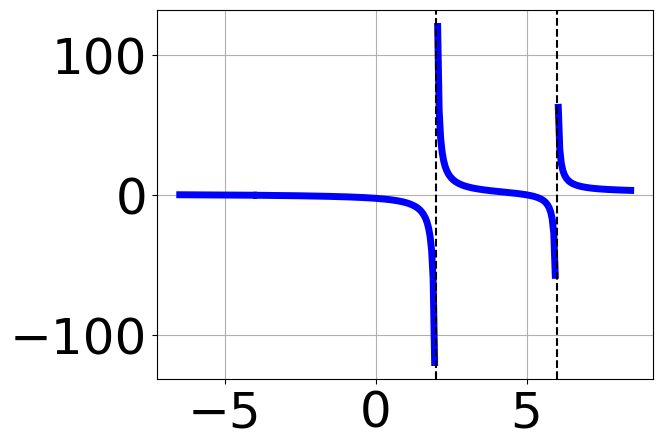
\includegraphics[width=0.5\textwidth]{../Figures/identifyGraphOfRationalFunctionCopyB.png}
\end{center}
\begin{enumerate}[label=\Alph*.]
\item \( f(x)=\frac{x^{3} -4 x^{2} -x + 4}{x^{3} +2 x^{2} -13 x + 10} \)
\item \( f(x)=\frac{x^{3} -1 x^{2} -16 x + 16}{x^{3} -2 x^{2} -13 x -10} \)
\item \( f(x)=\frac{x^{3} -4 x^{2} -x + 4}{x^{3} +2 x^{2} -13 x + 10} \)
\item \( f(x)=\frac{x^{3} +4 x^{2} -x -4}{x^{3} -2 x^{2} -13 x -10} \)
\item \( \text{None of the above are possible equations for the graph.} \)

\end{enumerate} }
\litem{
Determine the vertical asymptotes and holes in the rational function below.\[ f(x) = \frac{9x^{3} +12 x^{2} -17 x -20}{9x^{2} -6 x -8} \]\begin{enumerate}[label=\Alph*.]
\item \( \text{Holes at } x = -0.667 \text{ and } x = 1.333 \text{ with no vertical asymptotes.} \)
\item \( \text{Vertical Asymptote of } x = -0.667 \text{ and hole at } x = 1.333 \)
\item \( \text{Vertical Asymptotes of } x = -0.667 \text{ and } x = 1.333 \text{ with no holes.} \)
\item \( \text{Vertical Asymptote of } x = 1.0 \text{ and hole at } x = 1.333 \)
\item \( \text{Vertical Asymptotes of } x = -0.667 \text{ and } x = -1.667 \text{ with a hole at } x = 1.333 \)

\end{enumerate} }
\litem{
Determine the vertical asymptotes and holes in the rational function below.\[ f(x) = \frac{9x^{3} +42 x^{2} +16 x -32}{12x^{2} +x -20} \]\begin{enumerate}[label=\Alph*.]
\item \( \text{Vertical Asymptote of } x = 0.75 \text{ and hole at } x = -1.333 \)
\item \( \text{Vertical Asymptotes of } x = 1.25 \text{ and } x = 0.667 \text{ with a hole at } x = -1.333 \)
\item \( \text{Holes at } x = 1.25 \text{ and } x = -1.333 \text{ with no vertical asymptotes.} \)
\item \( \text{Vertical Asymptote of } x = 1.25 \text{ and hole at } x = -1.333 \)
\item \( \text{Vertical Asymptotes of } x = 1.25 \text{ and } x = -1.333 \text{ with no holes.} \)

\end{enumerate} }
\litem{
Determine the horizontal and/or oblique asymptotes in the rational function below.\[ f(x) = \frac{6x^{3} -5 x^{2} -34 x + 40}{3x^{2} +8 x -16} \]\begin{enumerate}[label=\Alph*.]
\item \( \text{Oblique Asymptote of } y = 2x -7. \)
\item \( \text{Horizontal Asymptote at } y = -4.0 \)
\item \( \text{Horizontal Asymptote of } y = 2.0  \)
\item \( \text{Horizontal Asymptote of } y = -4.0 \text{ and Oblique Asymptote of } y = 2x -7 \)
\item \( \text{Horizontal Asymptote of } y = 2.0 \text{ and Oblique Asymptote of } y = 2x -7 \)

\end{enumerate} }
\litem{
Determine the horizontal and/or oblique asymptotes in the rational function below.\[ f(x) = \frac{6x^{3} +11 x^{2} -17 x -30}{3x^{2} +x -10} \]\begin{enumerate}[label=\Alph*.]
\item \( \text{Horizontal Asymptote of } y = -2.0 \text{ and Oblique Asymptote of } y = 2x + 3 \)
\item \( \text{Horizontal Asymptote at } y = -2.0 \)
\item \( \text{Horizontal Asymptote of } y = 2.0 \text{ and Oblique Asymptote of } y = 2x + 3 \)
\item \( \text{Oblique Asymptote of } y = 2x + 3. \)
\item \( \text{Horizontal Asymptote of } y = 2.0  \)

\end{enumerate} }
\litem{
Which of the following functions \textit{could} be the graph below?
\begin{center}
    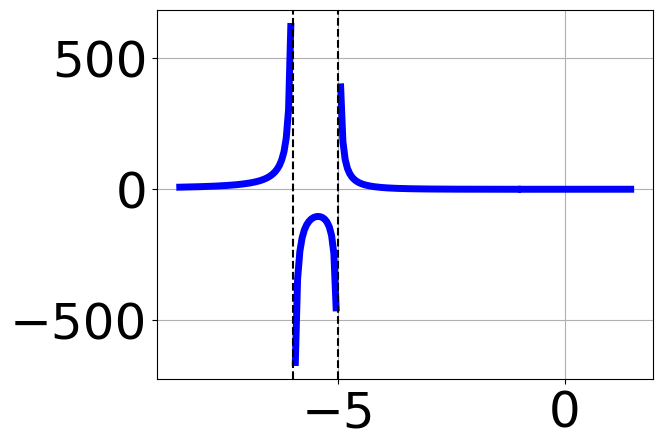
\includegraphics[width=0.5\textwidth]{../Figures/identifyGraphOfRationalFunctionB.png}
\end{center}
\begin{enumerate}[label=\Alph*.]
\item \( f(x)=\frac{x^{3} +10 x^{2} +33 x + 36}{x^{3} +8 x^{2} -13 x -140} \)
\item \( f(x)=\frac{x^{3} +3 x^{2} -16 x -48}{x^{3} +8 x^{2} -13 x -140} \)
\item \( f(x)=\frac{x^{3} -3 x^{2} -16 x + 48}{x^{3} -8 x^{2} -13 x + 140} \)
\item \( f(x)=\frac{x^{3} -3 x^{2} -16 x + 48}{x^{3} -8 x^{2} -13 x + 140} \)
\item \( \text{None of the above are possible equations for the graph.} \)

\end{enumerate} }
\litem{
Determine the vertical asymptotes and holes in the rational function below.\[ f(x) = \frac{9x^{3} +24 x^{2} +4 x -16}{9x^{2} +18 x + 8} \]\begin{enumerate}[label=\Alph*.]
\item \( \text{Holes at } x = -0.667 \text{ and } x = -1.333 \text{ with no vertical asymptotes.} \)
\item \( \text{Vertical Asymptotes of } x = -0.667 \text{ and } x = 0.667 \text{ with a hole at } x = -1.333 \)
\item \( \text{Vertical Asymptote of } x = -0.667 \text{ and hole at } x = -1.333 \)
\item \( \text{Vertical Asymptote of } x = 1.0 \text{ and hole at } x = -1.333 \)
\item \( \text{Vertical Asymptotes of } x = -0.667 \text{ and } x = -1.333 \text{ with no holes.} \)

\end{enumerate} }
\litem{
Determine the vertical asymptotes and holes in the rational function below.\[ f(x) = \frac{6x^{3} -13 x^{2} -9 x + 10}{9x^{2} -18 x + 8} \]\begin{enumerate}[label=\Alph*.]
\item \( \text{Vertical Asymptote of } x = 0.667 \text{ and hole at } x = 0.667 \)
\item \( \text{Holes at } x = 1.333 \text{ and } x = 0.667 \text{ with no vertical asymptotes.} \)
\item \( \text{Vertical Asymptotes of } x = 1.333 \text{ and } x = 2.5 \text{ with a hole at } x = 0.667 \)
\item \( \text{Vertical Asymptote of } x = 1.333 \text{ and hole at } x = 0.667 \)
\item \( \text{Vertical Asymptotes of } x = 1.333 \text{ and } x = 0.667 \text{ with no holes.} \)

\end{enumerate} }
\litem{
Determine the horizontal and/or oblique asymptotes in the rational function below.\[ f(x) = \frac{15x^{3} +61 x^{2} +72 x + 20}{20x^{3} +31 x^{2} +52 x + 12} \]\begin{enumerate}[label=\Alph*.]
\item \( \text{Horizontal Asymptote of } y = 0.750  \)
\item \( \text{Vertical Asymptote of } y = -2  \)
\item \( \text{None of the above} \)
\item \( \text{Horizontal Asymptote of } y = 0  \)
\item \( \text{Vertical Asymptote of } y = -0.750  \)

\end{enumerate} }
\end{enumerate}

\end{document}